% Template for taking notes\writing down exercise solutions
% In the specific context of mathematical Curricular Units

% In order to draw Finite State Machines\Turing Machines,
% we make use of the tikz-automata library
\documentclass[compress,svgnames,handout,13.7pt]{beamer}
\mode<presentation>
\usepackage[portuguese]{babel}
\usepackage{tikz}
\usetikzlibrary{automata, positioning, arrows}
\usepackage{makeidx,verbatim}
\usepackage{latexsym,amsfonts,amsmath,amssymb,amsthm}
\usepackage{curves}
\usepackage{enumerate}
\usepackage{moreverb}
\usepackage{cases}
\usepackage{array}
\usepackage{epsfig}
\usepackage{graphics}
\usepackage{float}
\usepackage{color}
%%\usepackage[latin1]{inputenc}
\usepackage{stmaryrd}
\usepackage{amstext}
\usepackage{xspace}
\usepackage[mathcal]{euscript}
\usepackage{rotating}
\usepackage{mathrsfs}
\usepackage{pgf,pgfnodes,pgfheaps}
\usepackage{listings}
\usepackage{xcolor}
\usetikzlibrary{arrows,automata,backgrounds}

\usecolortheme{seahorse}
\usecolortheme{rose}
\usefonttheme[onlylarge]{structuresmallcapsserif}
\setbeamerfont{frametitle}{family=\rmfamily,size=\footnotesize}
\setbeamercolor{title}{fg=blue!80!black}%,bg=blue!20!white}
\setbeamercolor{frametitle}{fg=blue!80!black}%,bg=blue!20!white}
\setbeamercolor{institute}{fg=blue!80!black}
\setbeamertemplate{miniframes}[tick]
\setbeamercovered{still covered={\opaqueness<1->{4}},
	again covered={\opaqueness<1->{4}}}
\setbeamerfont{small}{size=\small} \setbeamerfont{tiny}{size=\tiny}
\setbeamercolor{caixa}{fg=black,bg=blue!10!white}
\setbeamertemplate{navigation symbols}{}
\addtobeamertemplate{footline}
    {\leavevmode%
    \hbox{%
    \begin{beamercolorbox}
        [
        wd=\paperwidth,
        ht=2.75ex,
        dp=.5ex,
        right,
        rightskip=1em
        ]
        {mycolor}%
    \usebeamercolor[fg]{navigation symbols}
    \insertslidenavigationsymbol%
    \insertframenavigationsymbol%
    \insertsubsectionnavigationsymbol%
    \insertsectionnavigationsymbol%
    \insertdocnavigationsymbol%
    \insertbackfindforwardnavigationsymbol%
    \end{beamercolorbox}%
    }%
    \vskip0.5pt
 }{}

\def\N{{\mathbb N}}
\newcommand{\Z}{\mathbb Z}
\newcommand{\R}{\mathbb R}
\newcommand{\Q}{\mathbb Q}
\def\dotminus{\mathbin{\ooalign{\hss\raise1ex\hbox{.}\hss\cr\mathsurround=0pt$-$}}}
\def\proof{\noindent{\bf\blue Proof}\ }
			
\def\red{\color[rgb]{0.8,0,0}}
\def\lightred{\color[rgb]{1,0.5,0.5}}
\def\green{\color[rgb]{0,0.5,0}}
\def\lightgreen{\color[rgb]{0.5,1,0.5}}
\def\blue{\color[rgb]{0,0,0.7}}
\def\darkredblue{\color[rgb]{0.4,0,0.4}}
\def\lightgray{\color[rgb]{0.7,0.7,0.7}}
\def\mystep#1#2{\uncover<#1->{{\color<#1>[rgb]{0,0,1}{#2}}}}
\definecolor{azul}{rgb}{0,0,.7}
\definecolor{codegreen}{rgb}{0,0.6,0}
\definecolor{codegray}{rgb}{0.5,0.5,0.5}
\definecolor{codepurple}{rgb}{0.58,0,0.82}
\definecolor{backcolour}{rgb}{0.95,0.95,0.92}
\tikzset{->,
    >=stealth',
    node distance=3cm,
    every state/.style={thick, fill=gray!10},
    initial text=$ $,
}

\lstdefinestyle{mystyle}{backgroundcolor=\color{backcolour},
    commentstyle=\color{codegreen},
    keywordstyle=\color{magenta},
    numberstyle=\tiny\color{codegray},
    stringstyle=\color{codepurple},
    basicstyle=\ttfamily\footnotesize,
    breakatwhitespace=false,
    breaklines=true,
    captionpos=b,
    keepspaces=true,
    numbers=left,
    numbersep=5pt,
    showspaces=false,
    showstringspaces=false,
    showtabs=false,
    tabsize=2
}

\lstset{style=mystyle}

\renewcommand\qedsymbol{QED}


\title[Checkpoint]
    {\textbf{Mademoiselle Borges: Um Sistema de Bases de Dados para
Gestão de Eventos em Eventopolis\\
    \textbf{Grupo 06} \\
    \textit{Bases de Dados}}
}

\author[G06]{%
  \begin{tabular}{c}
    Bruno Gião \\
    A96544
  \end{tabular}
  \begin{tabular}{c}
    João Pereira \\
    A95375
  \end{tabular}
  \begin{tabular}{c}
    Helena Salazar \\
    A75635
  \end{tabular}
  \begin{tabular}{c}
    Tiago Teixeira \\
    A97666
  \end{tabular}
}


\date{\today}




\usetheme{CambridgeUS}
%\setbeamercovered{transparent}
\setbeamercovered{invisible}
\begin{document}


% Title Page
\thispagestyle{empty}
\frame{\titlepage}


% Table of Contents
\begin{frame}{Conteúdo}
\setcounter{secnumdepth}{2}
\setcounter{tocdepth}{2}
\tableofcontents
\end{frame}


\section{Introdução}

\subsection{Apresentação do Caso de Estudo}
\begin{frame}{Apresentação do Caso de Estudo}
Este trabalho consistirá então na elaboração de um SBD que consiga, aptamente, ajudar Henrique Borges
e a c\^amara municipal de Eventopolis a gerir e publicitar os seus eventos.
\end{frame}

\subsection{Estrutura do Relatório}
\begin{frame}{Estrutura do Relatório}
Após esta introdução, seguir-se-ão mais dois capítulos, nomeadamente, referentes à metodologia e à conclusão, seguido também de um capítulo complementar para potenciais anexos.
Na metodologia, teremos uma secção para cada fase do “ciclo de vida” do desenvolvimento
de bases de dados, isto é a, definição de requisitos e modelação conceptual.
\end{frame}

\section{Metodologia}

\subsection{Definição do Sistema}

\subsubsection{Contextualização}
\begin{frame}{Contextualização}
Em Eventopolis, uma localidade remota no centro de uma densa floresta, a gestão dos eventos sempre foi baseada em \textit{outsourcing} ou métodos manuais, devido à escassez de recursos humanos e à existência de um monopólio na área de Bases de Dados (BD). Este monopólio era controlado por uma seita de ocultistas tecnológicos, os quais praticavam preços exorbitantes e limitavam o acesso a uma parte significativa das informações nas suas bases de dados. Após uma revolta motivada pela insatisfação com a direção da empresa, alguns ex-membros, descontentes com a situação, optaram por adotar uma abordagem mais humanista e criar uma \textit{start-up} de Engenharia de Software em Eventopolis.
    
    Ao tomar conhecimento desta informação, o Professor Doutor Henrique Borges, responsável atual pela Gestão de Eventos na Câmara Municipal da cidade, prontamente identificou a oportunidade de mitigar os prejuízos significativos dos últimos anos ao estabelecer um contrato com a referida start-up para a implementação de um sistema de Bases de Dados \textit{open-source}.
\end{frame}
\begin{frame}{Contextualização}
 O sistema de Bases de Dados seria batizado de "Mademoiselle Borges" em homenagem a Antoinette Borges, a antiga gestora de Eventos da Câmara Municipal de Eventopolis e esposa de Henrique Borges, que faleceu há alguns anos. Antoinette enfrentou uma pressão considerável ao depender da seita ou ao ser forçada a gerir manualmente os eventos com uma equipa de funcionários bastante limitada, desafios que foram fatores cruciais para o seu falecimento precoce.
   
Para Henrique Borges, este projeto tem então um significado profundamente pessoal. Além de simplificar o funcionamento dos eventos, diminuindo a mortalidade deste posto de trabalho, a criação deste Sistema também reflete a sua vontade de fomentar a promoção da arte e da cultura na sua pequena cidade, algo que era o maior sonho da sua falecida esposa. Antoinette queria ver a transformação da modesta e isolada cidade numa capital cultural, uma aspiração que, infelizmente, apenas se concretizaria após o seu falecimento.
\end{frame}
\begin{frame}{Contextualização}
Durante todos os eventos aprovados pela Câmara a cidade será transformada num cenário requintado que exalta a estética do estilo \textit{Art Nouveau}, o estilo artístico predileto da Mademoiselle, este estilo tira inspiração da vegetação exuberante, densa e colorida, característica das imensas florestas que rodeiam Eventopolis. O principal local de eventos será uma gigantesca estufa situada no parque central, construída no início do século XX. Esta estrutura possui uma cúpula central e vitrais coloridos, com um esqueleto de ferro com linhas detalhadas e artísticas, que ao longo do tempo oxidaram e agora exibem uma tonalidade verde clássica.
\end{frame}

\subsubsection{Fundamentação}
\begin{frame}{Fundamentação}
Considerando o modo prévio de gerir eventos em Eventopolis, onde o uso de serviços externos era considerado excessivamente dispendioso, e diante da escassez de recursos humanos para uma gestão manual, a única alternativa viável, na perspetiva de Henrique Borges, seria desenvolver um SBD interno.
\end{frame}

\subsubsection{Objetivos}
\begin{frame}{Objetivos}
    O Professor Doutor Henrique Borges acredita que a introdu\c{c}\~{a}o de uma base de dados
    trar\'{a} sucesso aos eventos.

    Os objetivos mencionados abaixo s\~{a}o fundamentais para refletir este sucesso:
    \begin{itemize}
    \item Aumentar a capacidade de armazenamento de informa\c{c}\~{o}es;
    \item Saber em tempo real qual a previsão de afluência de cada evento, sendo assim possível
planear os eventos com maior precisão;
    \item Perceber quais são os colaboradores com melhor desempenho nas vendas, permitindo o
uso de incentivos para estimulá-los a alcançar novos patamares de vendas;
    \item Possibilitar uma gestão financeira mais abrangente e precisa;
    \item Garantir que é minimizada a possibilidade da capacidade do evento ser excedida;
    \end{itemize}
\end{frame}
\begin{frame}{Objetivos}
    \begin{itemize}
        \item Obter, em tempo real, um registo preciso das compras de cada participante, bem como
identificar os itens mais vendidos tanto em eventos específicos quanto globalmente;
        \item Melhorar a organiza\c{c}\~{a}o de hor\'{a}rios para cada evento;
        \item Promover a cidade em \^{a}mbito nacional e internacional;
        \item Estimular a economia local por meio de inje\c{c}\~{a}o de capital na regi\~{a}o;
    \end{itemize}
\end{frame}

\subsubsection{Viabilidade}
\begin{frame}{Viabilidade}
O Professor Doutor Henrique Borges defende que ao implementar um sistema de controlo de eventos
        será possível: 
        \begin{itemize}
          \item Recuperar, no final no primeiro semestre, $40\%$ das perdas anteriores e cerca de $20\%$
            do investimento inicial;
          \item Aumentar a participação nos eventos em $20\%$;
        \end{itemize}
\end{frame}

\subsubsection{Recursos a Utilizar}
\begin{frame}{Recursos a Utilizar}
Recursos Humanos:
\begin{itemize}
               \item Pessoal de limpeza;
               \item Equipa de seguran\c{c}a;
               \item Vendedores;
               \item Equipa de multim\'edia;
               \item Funcion\'{a}rios da empresa de desenvolvimento;
               \item Potenciais Volunt\'arios.
             \end{itemize}
Recursos Materiais:
\begin{itemize}
             \item{Hardware:}
               \begin{itemize}
                 \item 1 servidor fornecido pela \textit{start-up} com 128GiB;
                 \item 15 terminais ``burros'';
                 \item 10 computadores pessoais.
               \end{itemize}
             \item{Software:}
               \begin{itemize}
                 \item SGBD;
                 \item Aplicação de vendas e aprovisionamento;
                 \item Redes sociais para divulgar o calendários dos eventos.
               \end{itemize}
             \end{itemize}
\end{frame}

\subsubsection{Equipa de Trabalho}
\begin{frame}{Equipa de Trabalho}
\begin{itemize}
                 \item{\textbf{Pessoal Interno}}
                   Na equipa de gest\~ao de eventos da C\^amara Municipal de Eventopolis temos:
                   \begin{itemize}
                     \item{Professor Doutor Henrique Borges:} O coordenador principal da equipa;
                     \item{Maria Ivanovna Ivanova:} Empregada com experi\^encia em \textit{marketing} e co-coordenadora
                       da equipa;
                     \item{Herr Otto Mustermann:} Trabalhador \textit{part-time}.
                   \end{itemize}
                 \item{\textbf{Pessoal Externo}}
                   Já o pessoal externo, consiste na equipa de desenvolvimento da ``start-up'',
                   que seria constituída por 4 engenheiros, nomeadamente:
                   \begin{itemize}
                     \item Luke Bytespell
                     \item Aurelius Cibern\'etico
                     \item Bella Firewall
                     \item Aurora Matrix
                   \end{itemize}
             \end{itemize}
\end{frame}

\subsubsection{Plano de Execução do Trabalho}
\begin{frame}{Plano de Execução do Trabalho}
De forma a atempadamente desenvolver o SBD ``Mademoiselle Borges'', Henrique Borges e a equipa de desenvolvimento juntaram-se numa reuni\~ao e elaboraram o seguinte esquema GANTT:
\begin{figure}[h]
            \centering
            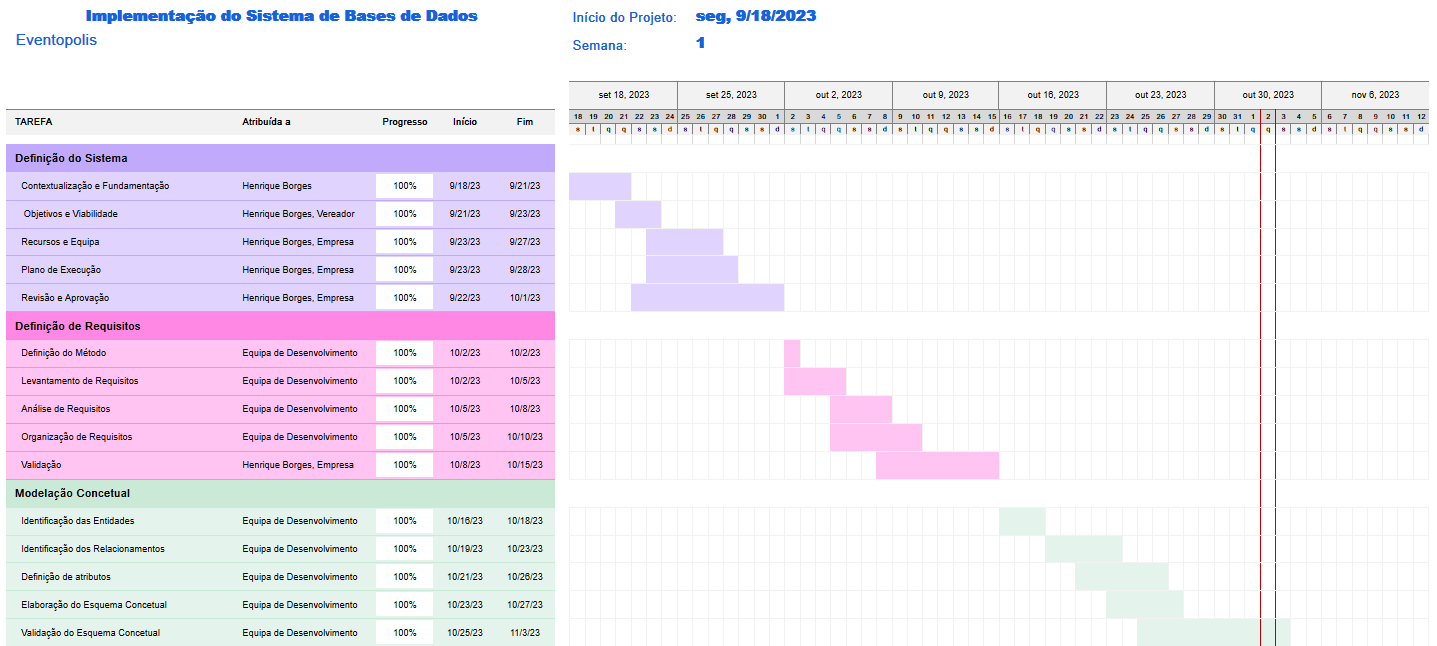
\includegraphics[width=4.75in]{images/GANTT1_c1.png}
            %%\caption{Diagrama de GANTT com conteúdos da primeira fase do Trabalho}
        \end{figure}
\end{frame}

\subsection{Definição de Requisitos}

\subsubsection{Método de Levantamento e de Análise de Requisitos Adotado}
\begin{frame}{Método de Levantamento e de Análise de Requisitos Adotado}
Com o objetivo de determinar os objetivos a serem alcançados pelo sistema de bases de dados, foram agendadas diversas reuniões com o Prof. D. Henrique Borges, onde foram discutidas várias questões pertinentes. No final destas reuniões, é previsto obter-se uma compreensão abrangente dos requisitos a serem implementados
\end{frame}

\subsubsection{Organização dos Requisitos Levantados}

\begin{frame}{Requisitos de Descrição}
\begin{table}[!ht]
    \centering
    \resizebox{\columnwidth}{!}{%
    \begin{tabular}{|l|l|l|>{\raggedright\arraybackslash}p{7cm}|l|l|l|}
    \hline
        Nr & ~ & Data e Hora & Descrição & Área & Fonte & Analista \\ \hline
        RD01 & 1 & 12:29 & Cada evento deve ter um identificador, uma descrição do mesmo, a data de início e de fim e pode ter, ou não, a capacidade & Eventos & Henrique Borges & Aurora Matrix \\ \hline
        RD02 & 2 & 12:30 & Cada funcionário deve ter um identificador, nome, NIF, data de nascimento, email, lista de telemoveis e morada (rua, localidade, código-postal & Eventos & Henrique Borges & Aurora Matrix \\ \hline
        RD03 & 3 & 12:31 & Cada venda deve ter um identificador, o valor total da venda, a quantidade de artigos na mesma e a data da venda & Eventos & Henrique Borges & Aurora Matrix \\ \hline
        RD04 & 4 & 12:32 & Cada participante dever ter um identificador, nome, NIF (opcional), data de nascimento, email (opcional), lista de números de telemóvel e opcionalmente, morada (rua, localidade, código-postal) & Eventos & Henrique Borges & Aurora Matrix \\ \hline
        RD05 & 5 & 12:33 & Cada artigo deve ter um identificador, nome, descrição do mesmo, preço e stock & Eventos & Henrique Borges & Aurora Matrix \\ \hline
        RD06 & 6 & 12:34 & Cada fornecedor deve ter um identificador, nome, IBAN, email, contacto (a pessoa que contactamos na empresa e o seu número de telemóvel), lista de números de telemóvel, morada (rua, localidade, código-postal) & Eventos & Henrique Borges & Aurora Matrix \\ \hline
    \end{tabular}%
    }
\end{table}
\end{frame}

\begin{frame}{Requisitos de Manipulação}
\begin{table}[!ht]
    \centering
    \resizebox{\columnwidth}{!}{%
    \begin{tabular}{|l|l|l|>{\raggedright\arraybackslash}p{8cm}|l|l|l|}
    \hline
        Nr & ~ & Data e Hora & Descrição & Área & Fonte & Analista \\ \hline
        RM01 & 10 & 12:37 & O administrador deve conseguir consultar qual funcionário gere qual & Eventos & Henrique Borges & Aurora Matrix \\ \hline
        RM02 & 11 & 12:38 & Um funcionário deve ser capaz de consultar qual é o funcionário que o gere & Eventos & Henrique Borges & Aurora Matrix \\ \hline
        RM03 & 12 & 12:39 & Um funcionário deve ser capaz de consultar que funcionário(s) gere & Eventos & Henrique Borges & Aurora Matrix \\ \hline
        RM04 & 13 & 12:40 & O administrador deve ser capaz de consultar as vendas efetuadas por um funcionário específico & Eventos & Henrique Borges & Aurora Matrix \\ \hline
        RM05 & 14 & 12:41 & O administrador deve ser capaz de consultar todas as vendas efetuadas & Eventos & Henrique Borges & Aurora Matrix \\ \hline
        RM06 & 15 & 12:42 & Um funcionário deve ser capaz de consultar as vendas que efetuou & Eventos & Henrique Borges & Aurora Matrix \\ \hline
        RM07 & 16 & 12:43 & O administrador deve ser capaz de consultar os artigos numa venda & Eventos & Henrique Borges & Aurora Matrix \\ \hline
        RM08 & 17 & 12:44 & O administrador deve ser capaz de consultar todos os artigos que estão numa venda & Eventos & Henrique Borges & Aurora Matrix \\ \hline
        RM09 & 18 & 12:45 & Um funcionário deve ser capaz de consultar os artigos numa venda & Eventos & Henrique Borges & Aurora Matrix \\ \hline
        RM10 & 19 & 12:46 & O administrador deve ser capaz de consultar todos os artigos & Eventos & Henrique Borges & Aurora Matrix \\ \hline
        RM11 & 20 & 12:47 & O administrador deve ser capaz de consultar os participantes de um evento & Eventos & Henrique Borges & Aurora Matrix \\ \hline
    \end{tabular}%
}
\end{table}
\end{frame}

\begin{frame}{Requisitos de Manipulação}
\begin{table}[!ht]
    \centering
    \resizebox{\columnwidth}{!}{%
    \begin{tabular}{|l|l|l|>{\raggedright\arraybackslash}p{8cm}|l|l|l|}
    \hline
        RM12 & 21 & 12:48 & O administrador deve ser capaz de consultar todos os participantes em todos os eventos & Eventos & Henrique Borges & Aurora Matrix \\ \hline
        RM13 & 22 & 12:49 & O administrador deve ser capaz de consultar o participante de uma venda específica & Eventos & Henrique Borges & Aurora Matrix \\ \hline
        RM14 & 23 & 12:50 & Um funcionário deve ser capaz de consultar o participante de uma venda que efetuou & Eventos & Henrique Borges & Aurora Matrix \\ \hline
        RM15 & 24 & 12:51 & O administrador deve ser capaz de consultar todas as vendas de um participante & Eventos & Henrique Borges & Aurora Matrix \\ \hline
        RM16 & 25 & 12:52 & O administrador deve ser capaz de consultar o fornecedor de um certo artigo & Eventos & Henrique Borges & Aurora Matrix \\ \hline
        RM17 & 26 & 12:53 & O administrador deve ser capaz de consultar os passados fornecedores de um certo artigo & Eventos & Henrique Borges & Aurora Matrix \\ \hline
        RM18 & 27 & 12:54 & O administrador deve ser capaz de consultar todos os fornecedores & Eventos & Henrique Borges & Aurora Matrix \\ \hline
        RM19 & 28 & 12:55 & O administrador deve ser capaz de consultar todos os funcionários & Eventos & Henrique Borges & Aurora Matrix \\ \hline
        RM20 & 29 & 12:56 & O administrador deve ser capaz de consultar todos os eventos & Eventos & Henrique Borges & Aurora Matrix \\ \hline
        RM21 & 30 & 12:57 & O administrador deve ser capaz de consultar o valor de vendas num dia particular & Eventos & Henrique Borges & Aurora Matrix \\ \hline
        RM22 & 31 & 12:58 & Deve ser possível determinar qual é o participante com maior valor de vendas & Eventos & Henrique Borges & Aurora Matrix \\ \hline
    \end{tabular}%
}
\end{table}
\end{frame}

\begin{frame}{Requisitos de Manipulação}
\begin{table}[!ht]
    \centering
    \resizebox{\columnwidth}{!}{%
    \begin{tabular}{|l|l|l|>{\raggedright\arraybackslash}p{8cm}|l|l|l|}
    \hline
        RM23 & 32 & 12:59 & Deve ser possível determinar qual é o evento com maior volume de vendas & Eventos & Henrique Borges & Aurora Matrix \\ \hline
        RM24 & 33 & 13:00 & Deve ser possível determinar qual foi o evento com maior participação & Eventos & Henrique Borges & Aurora Matrix \\ \hline
        RM25 & 34 & 13:01 & Os funcionários devem ser capazes de alterar as informações de um participante & Eventos & Henrique Borges & Aurora Matrix \\ \hline
        RM26 & 36 & 13:03 & No final do dia o sistema deve enviar um email ao Henrique Borges com o relatório de vendas & Eventos & Henrique Borges & Aurora Matrix \\ \hline
        RM27 & 37 & 13:04 & No final do dia o sistema deve enviar um email ao Henrique Borges com a afluência do evento & Eventos & Henrique Borges & Aurora Matrix \\ \hline
        RM28 & 38 & 13:05 & Um participante é inserido na base de dados quando compra um bilhete & Eventos & Henrique Borges & Aurora Matrix \\ \hline
        RM29 & 39 & 13:06 & Se o evento for gratuito a venda do bilhete deve ser registada na mesma mas com o valor a 0 & Eventos & Henrique Borges & Aurora Matrix \\ \hline
        RM30 & 40 & 13:07 & Não podem ser vendidos mais bilhetes para um evento do que a capacidade do mesmo & Eventos & Henrique Borges & Aurora Matrix \\ \hline
        RM31 & 42 & 13:09 & Os funcionários devem poder verificar o histórico de vendas de um participante & Eventos & Henrique Borges & Aurora Matrix \\ \hline
        RM32 & 44 & 13:12 & O administrador deve ser capaz de saber quais eventos decorreram num determinado período de tempo & Eventos & Henrique Borges & Aurora Matrix \\ \hline
        RM33 & 45 & 13:13 & O administrador deve ser capaz de consultar qual foi o funcionário que vendeu mais bilhetes num dado evento & Eventos & Henrique Borges & Aurora Matrix \\ \hline
    \end{tabular}%
}
\end{table}
\end{frame}

\begin{frame}{Requisitos de Controlo}
\begin{table}[!ht]
    \centering
    \resizebox{\columnwidth}{!}{%
    \begin{tabular}{|l|l|l|>{\raggedright\arraybackslash}p{8cm}|l|l|l|}
    \hline
        Nr & ~ & Data e Hora & Descrição & Área & Fonte & Analista \\ \hline
        RC01 & 7 & 12:35 & O administrador do sistema é o Henrique Borges & Eventos & Henrique Borges & Aurora Matrix \\ \hline
        RC02 & 8 & 12:36 & Herr Otto Mustermann e Maria Ivanovna Ivanova são também administradores & Eventos & Henrique Borges & Aurora Matrix \\ \hline
        RC03 & 9 & 12:36 & Herr Mustermann só tem acesso à base de dados entre as 15:30 e as 19:30 & Eventos & Henrique Borges & Aurora Matrix \\ \hline
        RC04 & 35 & 13:02 & Os funcionários não devem ter acesso ao valor de vendas de cada evento & Eventos & Henrique Borges & Aurora Matrix \\ \hline
        RC05 & 41 & 13:08 & O acesso à base de dados só está disponível das 07:00 às 02:00 & Eventos & Henrique Borges & Aurora Matrix \\ \hline
        RC06 & 43 & 13:10 & Os funcionários só podem aceder à base de dados se um evento estiver a decorrer & Eventos & Henrique Borges & Aurora Matrix \\ \hline
    \end{tabular}%
}
\end{table}
\end{frame}

\subsubsection{Análise e Validação Geral dos Requisitos}
\begin{frame}{Análise e Validação Geral dos Requisitos}
Depois do levantamento dos requisitos, marcou-se uma reunião no intuito de o pessoal externo tomar conhecimento dos requisitos documentados.

Essa reunião, por sua vez, foi realizada com sucesso, e o pessoal externo mostrou-se satisfeito com o progresso e nível de detalhe a que os membros da equipa de desenvolvimento de BD chegaram, especialmente o Prof. Dr. Henrique Borges, que viu muito potencial neste projeto.
\end{frame}

\subsection{Modelação Concetual}
\begin{frame}{Modelação Concetual}
\end{frame}

\subsubsection{Apresentação da abordagem de modelação realizada}
\begin{frame}{Apresentação da abordagem de modelação realizada}
\end{frame}

\subsubsection{Identificação e Caracterização das Entidades}
\begin{frame}{Identificação e Caracterização das Entidades}
\end{frame}

\subsubsection{Identificação e Caracterização da Associação dos Atributos com as Entidades e Relacionamentos}
\begin{frame}{Identificação e Caracterização da Associação dos Atributos com as Entidades e Relacionamentos}
\end{frame}

\subsubsection{Apresentação e Explicação do Diagrama ER Produzido}
\begin{frame}{Apresentação e Explicação do Diagrama ER Produzido}
\begin{figure}[h]
            \centering
            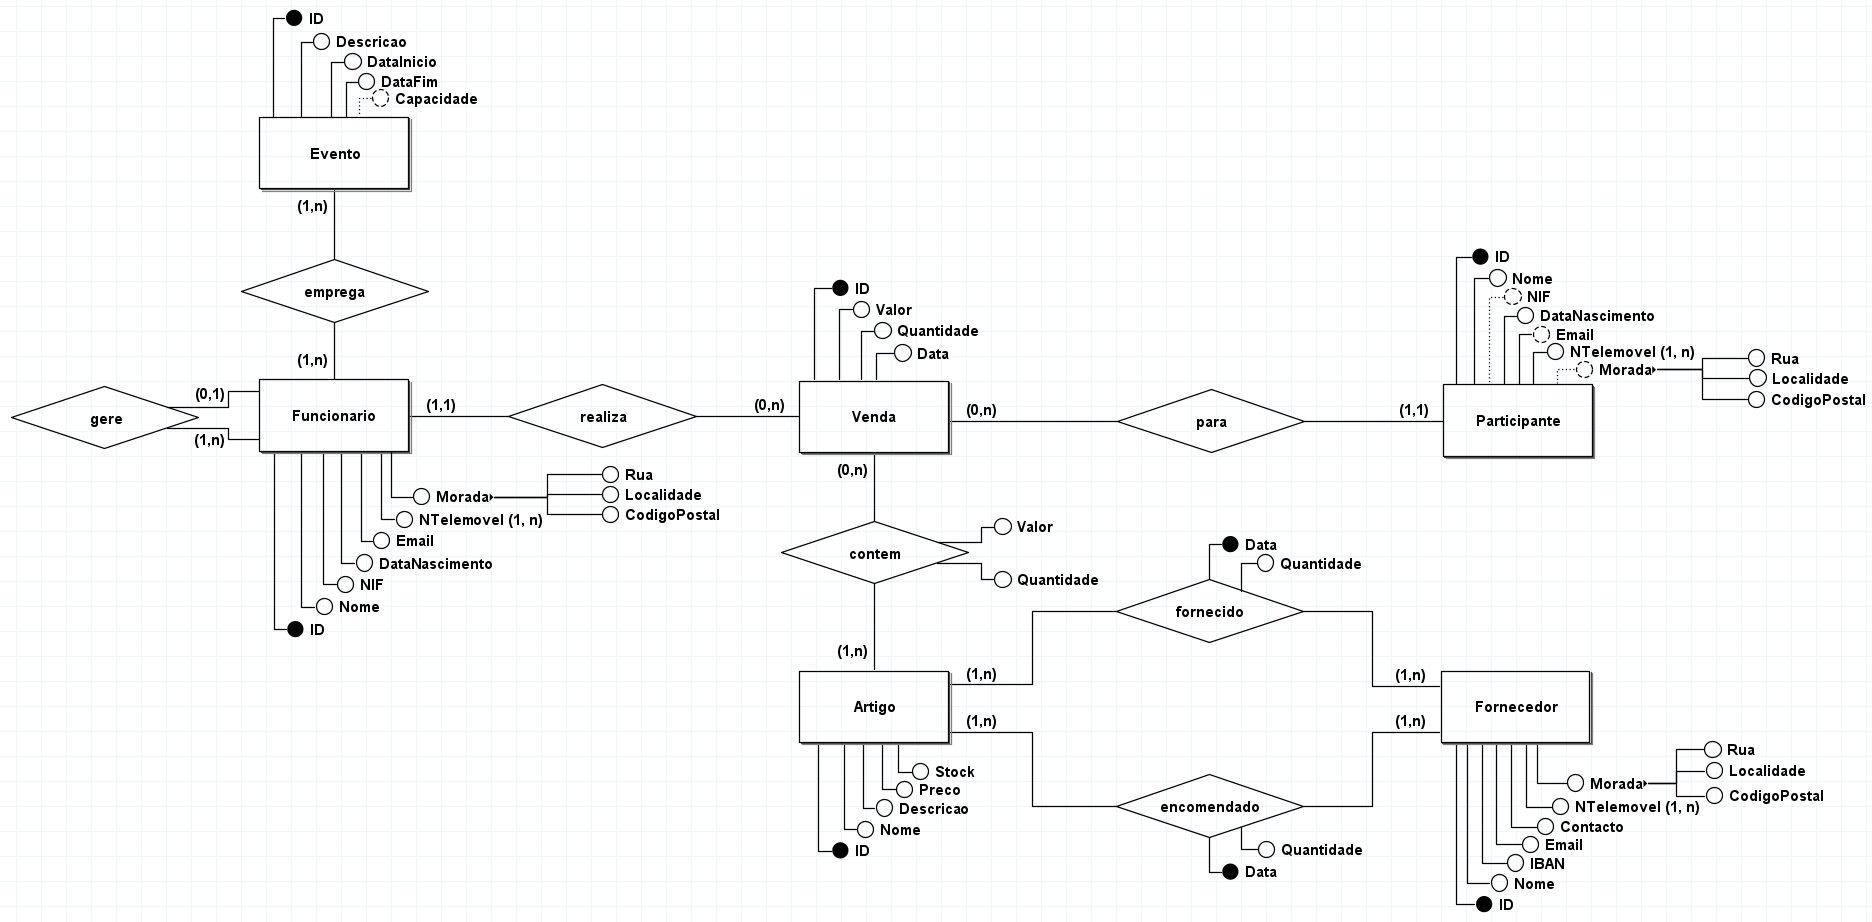
\includegraphics[width=4.75in]{images/Conceitual_Com_Atributos.png}
            %%\caption{Diagrama Conceitual}
        \end{figure}
\end{frame}

\section{Conclusão}
\begin{frame}{Conclusão}
\end{frame}

\thispagestyle{empty}
\frame{\titlepage}

\end{document}